% directive: erasureCodeInstancesFigure
% aria-label: Erasure code definition and its instances: Reed-Solomon over a field F, Reed-Solomon over F_{2^16} with N = 2^16 points, parallel Reed-Solomon over F^16, which uses Reed-Solomon, and the SPQR erasure code over F_{2^16}^16, which uses Reed-Solomon over F_{2^16}.
\documentclass[tikz,border=6pt]{standalone}
\usepackage[T1]{fontenc}
\usepackage{amsmath,amssymb}
\renewcommand{\familydefault}{\sfdefault}
\usepackage[eulergreek]{sansmath}
\sansmath
\usepackage{xcolor}
\usepackage{tikz}
\usetikzlibrary{positioning,calc,arrows.meta,fit,backgrounds,decorations.pathreplacing}
\definecolor{commentcolor}{HTML}{666666}
\definecolor{signalblue}{HTML}{3A76F0}
\definecolor{signalgreen}{HTML}{2A7B7B}
\definecolor{signalolive}{HTML}{4E7F60}
\definecolor{signalpurple}{HTML}{6B3FA0}
\definecolor{adversaryred}{HTML}{B42318}
\newcommand{\Encode}{\mathsf{Encode}}
\newcommand{\Decode}{\mathsf{Decode}}
\tikzset{
  panel/.style={draw=gray!45, line width=0.5pt, rounded corners=4pt, fill=gray!3, inner sep=6pt},
  algbox/.style={draw=signalolive!80, line width=0.7pt, rounded corners=3pt, fill=signalolive!10,
    inner sep=6pt, font=\small\sffamily, align=center},
  statebox/.style={draw=signalblue!70, line width=0.65pt, rounded corners=4pt, fill=signalblue!6,
    inner sep=6pt, font=\small\sffamily, align=center},
  keypill/.style={draw=signalpurple!75, line width=0.6pt, rounded corners=7pt, fill=signalpurple!9,
    inner xsep=8pt, inner ysep=4pt, font=\small\sffamily},
  chunk/.style={draw=signalblue!75, line width=0.55pt, rounded corners=2pt, fill=signalblue!9,
    minimum width=0.62cm, minimum height=0.50cm, inner sep=1pt, font=\scriptsize\sffamily},
  chunklost/.style={chunk, draw=gray!45, fill=gray!10, text=gray!55},
  sourcechunk/.style={chunk, draw=signalpurple!70, fill=signalpurple!9},
  goodpill/.style={draw=signalgreen!80, line width=0.65pt, rounded corners=7pt, fill=signalgreen!9,
    inner xsep=8pt, inner ysep=4pt, font=\small\sffamily},
  failpill/.style={draw=adversaryred!75, line width=0.65pt, rounded corners=7pt, fill=adversaryred!7,
    inner xsep=8pt, inner ysep=4pt, font=\small\sffamily},
  flow/.style={->, >=Stealth, line width=0.8pt, black},
  lossy/.style={->, >=Stealth, line width=0.5pt, gray!55, dashed},
  slot/.style={draw=gray!60, line width=0.5pt, minimum width=0.42cm, minimum height=0.42cm, inner sep=0pt},
  slotfull/.style={slot, fill=signalgreen!25, draw=signalgreen!70},
  slotempty/.style={slot, fill=white},
  lbl/.style={font=\small\sffamily, inner sep=2pt},
  slbl/.style={font=\scriptsize\sffamily, inner sep=1.5pt},
  note/.style={font=\scriptsize\sffamily\itshape, text=commentcolor, inner sep=1.5pt},
  theorybox/.style={draw=signalgreen!80, line width=0.8pt, rounded corners=4pt, fill=signalgreen!8,
    inner sep=7pt, font=\small\sffamily, align=center},
  instancebox/.style={draw=signalblue!70, line width=0.7pt, rounded corners=4pt, fill=signalblue!6,
    inner sep=7pt, font=\small\sffamily, align=center},
  instof/.style={->, >=Stealth, line width=0.8pt, black},
  uses/.style={->, >=Stealth, line width=0.7pt, dashed, signalolive},
  ecbox/.style={draw=signalblue!70, line width=0.7pt, rounded corners=3pt, fill=signalblue!7,
    inner sep=6pt, font=\small\sffamily, align=center},
  rolepill/.style={fill=signalgreen, text=white, rounded corners=5pt, inner xsep=9pt, inner ysep=4pt,
    font=\sffamily\bfseries},
  advpill/.style={draw=adversaryred!80, line width=0.7pt, rounded corners=5pt, fill=adversaryred!7,
    text=adversaryred, minimum width=1.05cm, minimum height=0.68cm, inner sep=3pt, font=\normalsize},
  timeline/.style={-, line width=0.6pt, gray!55},
}
\newcommand{\tagsf}[1]{{\scriptsize\sffamily\itshape\textcolor{commentcolor}{#1}}}
\newcommand{\notesf}[1]{{\scriptsize\sffamily\itshape\textcolor{signalpurple}{#1}}}

\begin{document}
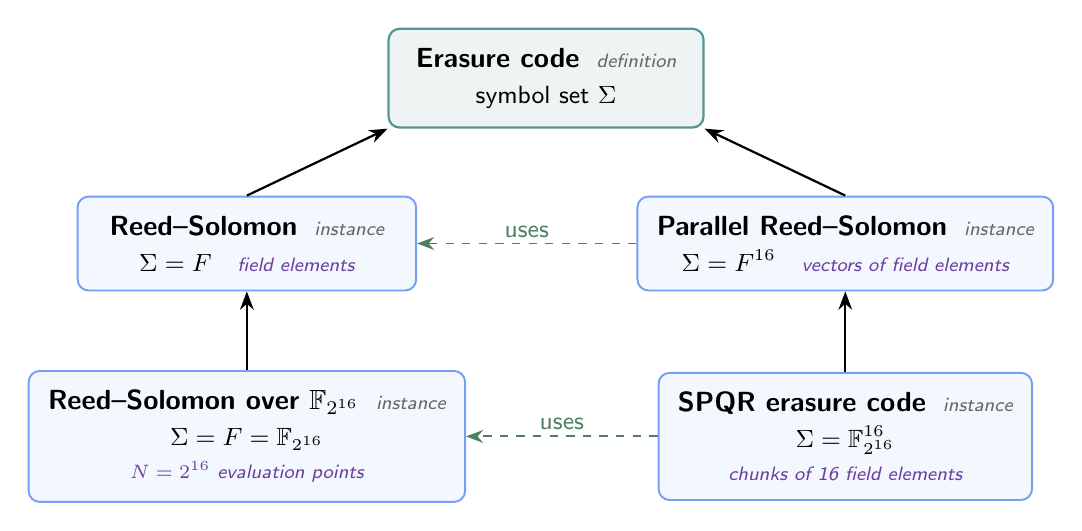
\begin{tikzpicture}[x=1cm,y=1cm]
  \node[theorybox, minimum width=4.00cm, minimum height=1.05cm] at (0,2.25) (ec)
    {{\normalsize\bfseries Erasure code}\ \ \tagsf{definition}\\[2pt] symbol set $\Sigma$};
  \node[instancebox, minimum width=4.30cm, minimum height=1.15cm] at (-3.80,0.15) (rs)
    {{\normalsize\bfseries Reed--Solomon}\ \ \tagsf{instance}\\[2pt]
     $\Sigma=F$\quad \notesf{field elements}};
  \draw[instof] (rs.north) -- (ec.south west);
  \node[instancebox, minimum width=4.30cm, minimum height=1.15cm] at (-3.80,-2.30) (crs)
    {{\normalsize\bfseries Reed--Solomon over $\mathbb F_{2^{16}}$}\ \ \tagsf{instance}\\[2pt]
     $\Sigma=F=\mathbb F_{2^{16}}$\\[1pt] \notesf{$N=2^{16}$ evaluation points}};
  \draw[instof] (crs.north) -- (rs.south);
  \node[instancebox, minimum width=4.30cm, minimum height=1.15cm] at (3.80,0.15) (prs)
    {{\normalsize\bfseries Parallel Reed--Solomon}\ \ \tagsf{instance}\\[2pt]
     $\Sigma=F^{16}$\quad \notesf{vectors of field elements}};
  \draw[instof] (prs.north) -- (ec.south east);
  \draw[uses] (prs.west) -- node[midway, above, lbl, signalolive] {uses} (rs.east);
  \node[instancebox, minimum width=4.60cm, minimum height=1.15cm] at (3.80,-2.30) (cprs)
    {{\normalsize\bfseries SPQR erasure code}\ \ \tagsf{instance}\\[2pt]
     $\Sigma=\mathbb F_{2^{16}}^{16}$\\[1pt] \notesf{chunks of 16 field elements}};
  \draw[instof] (cprs.north) -- (prs.south);
  \draw[uses] (cprs.west) -- node[midway, above, lbl, signalolive] {uses} (crs.east);
\end{tikzpicture}
\end{document}
